% Stanford EE364B Final Project Poster
% Differentiable Inverse DC-OPF
% Carlo Schreiber, Spring 2025
%
% Compile with: pdflatex poster.tex
% Requires: beamerposter package (texlive-latex-extra or MiKTeX)
%
% Poster size: 48in x 36in (standard landscape)

\documentclass[final]{beamer}

\usepackage[
  orientation=landscape,
  size=custom,
  width=121.92,   % 48 inches in cm
  height=91.44,   % 36 inches in cm
  scale=1.4
]{beamerposter}

\usepackage{amsmath,amssymb,amsthm}
\usepackage{graphicx}
\usepackage{booktabs}
\usepackage{xcolor}
\usepackage{multicol}
\usepackage{tikz}
\usepackage{tcolorbox}
\usepackage{microtype}
\usepackage{array}
\usepackage{ragged2e}

% -----------------------------------------------------------------------
% Stanford color palette (official)
% -----------------------------------------------------------------------
\definecolor{StanfordCardinal}{HTML}{8C1515}
\definecolor{StanfordDark}{HTML}{820000}
\definecolor{StanfordPaloAlto}{HTML}{175E54}
\definecolor{StanfordWarm}{HTML}{B83A4B}
\definecolor{StanfordSandstone}{HTML}{D2C295}
\definecolor{StanfordLightSand}{HTML}{F9F6EF}
\definecolor{StanfordGray}{HTML}{585754}
\definecolor{StanfordLightGray}{HTML}{EEEEEE}
\definecolor{blockbg}{HTML}{F5F0EB}

% -----------------------------------------------------------------------
% Beamer theme overrides
% -----------------------------------------------------------------------
\usetheme{default}
\setbeamercolor{background canvas}{bg=white}
\setbeamercolor{headline}{fg=white, bg=StanfordCardinal}
\setbeamercolor{footline}{fg=white, bg=StanfordDark}
\setbeamercolor{separation line}{bg=StanfordCardinal}
\setbeamercolor{block title}{fg=white, bg=StanfordCardinal}
\setbeamercolor{block body}{fg=black, bg=blockbg}
\setbeamercolor{block title alerted}{fg=white, bg=StanfordPaloAlto}
\setbeamercolor{block body alerted}{fg=black, bg=StanfordLightSand}
\setbeamercolor{normal text}{fg=black}
\setbeamerfont{block title}{size=\large, series=\bfseries}
\setbeamerfont{headline title}{size=\Huge, series=\bfseries}
\setbeamerfont{footline}{size=\normalsize}

% Remove navigation symbols
\setbeamertemplate{navigation symbols}{}

% -----------------------------------------------------------------------
% Custom headline
% -----------------------------------------------------------------------
\setbeamertemplate{headline}{
  \begin{beamercolorbox}[wd=\paperwidth]{headline}
    \vskip0.8cm
    \begin{columns}[T,onlytextwidth]
      % Left: Stanford logo area
      \begin{column}{0.14\paperwidth}
        \centering\vskip0.3cm
        % Stanford "S" block mark
        \begin{tikzpicture}
          \fill[StanfordDark] (0,0) rectangle (3.2,3.2);
          \node[text=white, font=\fontsize{52}{52}\selectfont\bfseries] at (1.6,1.6) {S};
        \end{tikzpicture}\\[0.3cm]
        {\color{white}\large\textbf{Stanford University}}\\
        {\color{StanfordSandstone}\normalsize Department of\\Electrical Engineering}
      \end{column}
      % Center: title + authors
      \begin{column}{0.70\paperwidth}
        \centering
        {\fontsize{52}{60}\selectfont\bfseries\color{white}
          Differentiable Inverse DC-OPF:\\[0.2cm]
          Recovering Generator Costs and Capacities from Dispatch Data}\\[0.6cm]
        {\large\color{StanfordSandstone}
          \textbf{Carlo Schreiber} \quad\textbullet\quad EE 364B Final Project \quad\textbullet\quad Stanford University \quad\textbullet\quad Spring 2025}
      \end{column}
      % Right: course badge
      \begin{column}{0.14\paperwidth}
        \centering\vskip0.4cm
        \begin{tikzpicture}
          \fill[StanfordDark, rounded corners=12pt] (0,0) rectangle (5.8,4.2);
          \node[text=white, align=center, font=\large\bfseries] at (2.9,3.0) {EE 364B};
          \node[text=StanfordSandstone, align=center, font=\normalsize] at (2.9,2.1) {Convex Optimization};
          \node[text=StanfordSandstone, align=center, font=\normalsize] at (2.9,1.35) {II};
          \node[text=white, align=center, font=\small] at (2.9,0.55) {Spring 2025};
        \end{tikzpicture}
      \end{column}
    \end{columns}
    \vskip0.6cm
    \begin{beamercolorbox}[wd=\paperwidth, ht=0.15cm]{separation line}\end{beamercolorbox}
  \end{beamercolorbox}
}

% -----------------------------------------------------------------------
% Custom footline
% -----------------------------------------------------------------------
\setbeamertemplate{footline}{
  \begin{beamercolorbox}[wd=\paperwidth, ht=1.8cm, leftskip=1.2cm, rightskip=1.2cm]{footline}
    \vskip0.4cm
    \begin{columns}[T]
      \begin{column}{0.5\paperwidth}
        {\small\color{white}
          \textbf{Code \& experiments:} \texttt{github.com/carlo-scr/ee364bfinal} \qquad
          \textbf{Solver:} cvxpylayers + SCS \quad \textbf{Optimizer:} Adam + cosine LR decay}
      \end{column}
      \begin{column}{0.5\paperwidth}
        \raggedleft
        {\small\color{StanfordSandstone}
          Key references: Keshavarz, Wang \& Boyd (2011) \textbullet\
          Agrawal et al.\ (2019) \textbullet\
          Fuentes-Valenzuela \& Degleris (2024)}
      \end{column}
    \end{columns}
  \end{beamercolorbox}
}

% -----------------------------------------------------------------------
% Block style with colored left rule
% -----------------------------------------------------------------------
\setbeamertemplate{block begin}{
  \vskip0.5cm
  \begin{beamercolorbox}[rounded=true, shadow=false, leftskip=0.5cm, rightskip=0.5cm,
                          ht=2.2ex, dp=1ex, colsep*=0ex]{block title}%
    \usebeamerfont{block title}\insertblocktitle
  \end{beamercolorbox}
  \vskip-0.5pt
  \usebeamercolor{block body}
  \begin{beamercolorbox}[rounded=true, shadow=false,
                          leftskip=0.5cm, rightskip=0.5cm, vmode]{block body}%
    \vskip0.5cm
}
\setbeamertemplate{block end}{
    \vskip0.4cm
  \end{beamercolorbox}
  \vskip0.4cm
}

\setbeamertemplate{block alerted begin}{
  \vskip0.5cm
  \begin{beamercolorbox}[rounded=true, shadow=false, leftskip=0.5cm, rightskip=0.5cm,
                          ht=2.2ex, dp=1ex]{block title alerted}%
    \usebeamerfont{block title}\insertblocktitle
  \end{beamercolorbox}
  \vskip-0.5pt
  \usebeamercolor{block body alerted}
  \begin{beamercolorbox}[rounded=true, shadow=false,
                          leftskip=0.5cm, rightskip=0.5cm, vmode]{block body alerted}%
    \vskip0.5cm
}
\setbeamertemplate{block alerted end}{
    \vskip0.4cm
  \end{beamercolorbox}
  \vskip0.4cm
}

% -----------------------------------------------------------------------
% Convenience macros
% -----------------------------------------------------------------------
\newcommand{\R}{\mathbb{R}}
\newcommand{\opt}{^{\star}}
\newcommand{\hatp}[1]{\hat{#1}}
\newcommand{\highlight}[1]{\textcolor{StanfordCardinal}{\textbf{#1}}}
\newcommand{\paloalto}[1]{\textcolor{StanfordPaloAlto}{\textbf{#1}}}

% -----------------------------------------------------------------------
\begin{document}
\begin{frame}[t]{}

\vskip0.3cm
\begin{columns}[t, totalwidth=\textwidth]

%% =====================================================================
%% COLUMN 1
%% =====================================================================
\begin{column}{0.305\textwidth}

  % --- Motivation ---------------------------------------------------
  \begin{block}{Motivation \& Problem}
    Power-system operators publish enormous quantities of dispatch data
    (hourly generation, demand, clearing prices) \textbf{without disclosing}
    underlying cost curves or operating limits.
    \medskip

    Recovering these latent parameters is central to:
    \begin{itemize}
      \item \textbf{Marginal emission factor (MEF)} forecasting
      \item Counterfactual policy analysis
      \item Calibrating capacity-expansion models
      \item Detecting market power
    \end{itemize}

    \medskip
    \begin{tcolorbox}[colback=StanfordLightSand, colframe=StanfordCardinal,
                      boxrule=1.5pt, arc=4pt, left=4pt, right=4pt]
      \textbf{Goal:} Given $T$ demand--dispatch pairs
      $\{(d_t,\, g_t)\}_{t=1}^T$ produced by an unknown DC-OPF, recover
      \[
        \theta\opt = \bigl(f\opt,\; g_{\max}\opt,\; p_{\max}\opt\bigr).
      \]
    \end{tcolorbox}
  \end{block}

  % --- Forward model ------------------------------------------------
  \begin{block}{Forward DC-OPF}
    For incidence $A\in\R^{n\times m}$, the DC optimal power flow is:
    \[
    \begin{aligned}
      \min_{g,p,\theta}\;&
        f^\top g + \tfrac{\varepsilon}{2}\|g\|_2^2 + \tfrac{\tau}{2}\|p\|_2^2\\
      \text{s.t.}\;& Ap + g = d \\
      & p = \mathrm{diag}(b)\,A^\top\theta \\
      & 0 \le g \le g_{\max},\quad |p|\le p_{\max}
    \end{aligned}
    \]

    Tikhonov regularizers ($\varepsilon{=}0.1$, $\tau{=}0.01$) make the
    QP \textbf{strongly convex}, so the solution map
    $(d, f, g_{\max}, p_{\max}) \mapsto (g\opt, p\opt)$ is unique and
    Lipschitz-differentiable.

    \medskip
    \textcolor{StanfordGray}{\small Setting $b\equiv1$ gives a
    network-flow relaxation; the physics can be tightened with real
    susceptances as needed.}
  \end{block}

  % --- Identifiability ----------------------------------------------
  \begin{block}{Active-Set Identifiability}
    A generator's cost is observable \emph{only} when its dispatch is
    sensitive to demand changes.

    \medskip
    \textbf{Lemma.} \textit{Fix $(d,g_{\max},p_{\max})$.  If generator
    $i$ is strictly interior ($0 < g_i\opt < g_{\max,i}$) and the KKT
    system is non-degenerate, then $\partial g_i\opt/\partial f_i \neq 0$.
    Conversely, if generator $i$ is at a bound for all $t$, then $f_i$
    is unidentifiable from $\{(d_t,g_t)\}$.}

    \medskip
    \textbf{Empirical identifiability score:}
    \[
      s_i \;=\; \frac{1}{T}\sum_{t=1}^T
      \mathbf{1}\!\bigl[\mathrm{tol}\le g_{t,i}\opt \le g_{\max,i}-\mathrm{tol}\bigr]
    \]

    \begin{center}
      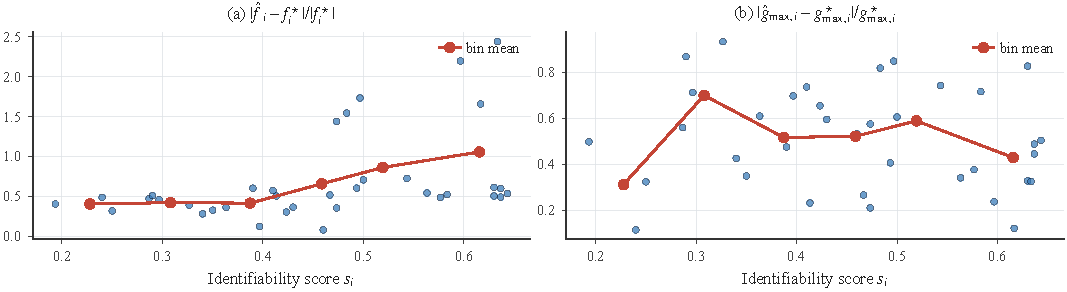
\includegraphics[width=0.92\linewidth]{../paper/figures/identifiability.pdf}
    \end{center}
    {\small Per-generator recovery error vs.\ identifiability score.
    High-$s_i$ generators (strictly interior) are reliably recovered;
    always-binding generators concentrate at high error.}
  \end{block}

\end{column}

%% =====================================================================
%% COLUMN 2
%% =====================================================================
\begin{column}{0.375\textwidth}

  % --- Inverse estimation -------------------------------------------
  \begin{block}{Differentiable Inverse Estimator}
    We embed the forward QP in a \texttt{CvxpyLayer} and minimize:

    \[
      \mathcal{L}(\hat\theta) =
        \frac{1}{T}\sum_{t=1}^T
          \mathrm{Huber}\!\bigl(g\opt(d_t;\hat\theta) - g_t^{\mathrm{obs}}\bigr)
        + \lambda_2\|\hat\theta\|_2^2
        + \lambda_L\,\mathrm{Lap}(\hat F)
    \]

    \begin{itemize}
      \item $\hat\theta = (\hat f,\hat g_{\max},\hat p_{\max})$ via softplus
            parameterization (enforces non-negativity)
      \item $\hat F\in\R^{S\times n}$: stratified cost table (one cost
            vector per hour-of-day stratum $s$)
      \item $\mathrm{Lap}(\hat F) = \mathrm{tr}(\hat F^\top L\hat F)$:
            cycle Laplacian regularizes hour-to-hour drift
      \item Gradients $\nabla_{\hat\theta} g\opt$ via implicit KKT
            differentiation (cvxpylayers)
      \item Optimizer: Adam + cosine LR decay + early stopping
    \end{itemize}

    \medskip
    \textbf{Three extensions over the F\&D baseline:}
    \vspace{2pt}

    \begin{tabular}{@{}c p{0.80\linewidth}@{}}
      \textcolor{StanfordCardinal}{\large\textbf{1}} &
        \textbf{Extended parameters.} Jointly learn $(f, g_{\max}, p_{\max})$
        — not just costs. \\[4pt]
      \textcolor{StanfordCardinal}{\large\textbf{2}} &
        \textbf{Stratified costs.} Laplacian-regularized per-stratum
        $f^{(s)}$ captures diurnal merit-order swing. \\[4pt]
      \textcolor{StanfordCardinal}{\large\textbf{3}} &
        \textbf{Robust loss.} Huber residual tolerates sensor noise,
        derates, and unit-commitment effects. \\
    \end{tabular}
  \end{block}

  % --- Headline results table ---------------------------------------
  \begin{alertblock}{Headline Results — 10-Bus Synthetic Benchmark}
    {\small 3 seeds, mean $\pm$ std. \textit{Diff.} rows = this work.
    Clean NRMSE: forward error on noise-free GT dispatch.}

    \medskip
    \renewcommand{\arraystretch}{1.25}
    \begin{tabular}{@{}lcccc@{}}
      \toprule
      \textbf{Method} &
        \textbf{NRMSE}$_\text{cl.}$ &
        $\boldsymbol{\cos\hat f}$ &
        \textbf{Merit acc.} &
        $\boldsymbol{\cos\hat g_{\max}}$ \\
      \midrule
      Ridge         & 0.110 & ---               & ---               & --- \\
      MLP           & 0.477 & ---               & ---               & --- \\
      KKT baseline  & 0.138 & $.908{\pm}.019$   & $.881{\pm}.034$   & $.870{\pm}.055$ \\
      \midrule
      \highlight{Diff.\ (caps fixed)} &
        \highlight{0.125} &
        \highlight{$.959{\pm}.012$} &
        \highlight{$.904{\pm}.013$} &
        \highlight{$1.00$} \\
      Diff.\ (full) & 0.208 & $.949{\pm}.018$   & $.889{\pm}.022$   & $.999$ \\
      Diff.\ (strat.)& 0.198 & $.947{\pm}.018$  & $.874{\pm}.046$   & $.999$ \\
      \bottomrule
    \end{tabular}

    \bigskip
    \begin{center}
      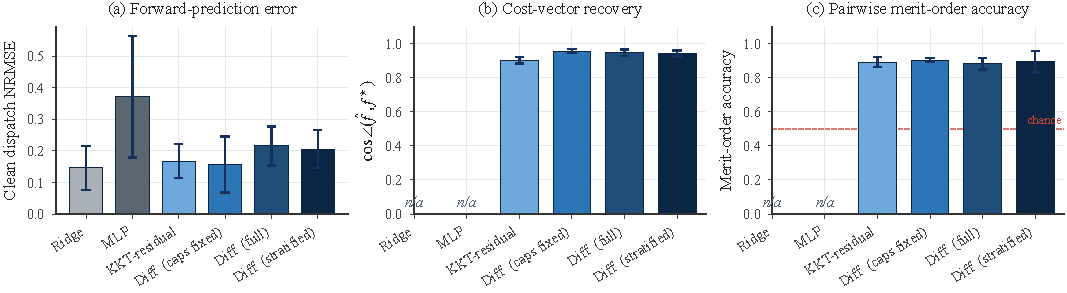
\includegraphics[width=0.96\linewidth]{../paper/figures/methods_comparison.pdf}
    \end{center}
    {\small \textbf{(a)} Clean dispatch NRMSE. \textbf{(b)} Cosine recovery of
    $\hat f$. \textbf{(c)} Merit-order accuracy.  Regression baselines
    (Ridge, MLP) overfit noise and recover \emph{no} structural parameters.}
  \end{alertblock}

  % --- Methods comparison deep dive ---------------------------------
  \begin{block}{Parameter Recovery Detail}
    \begin{center}
      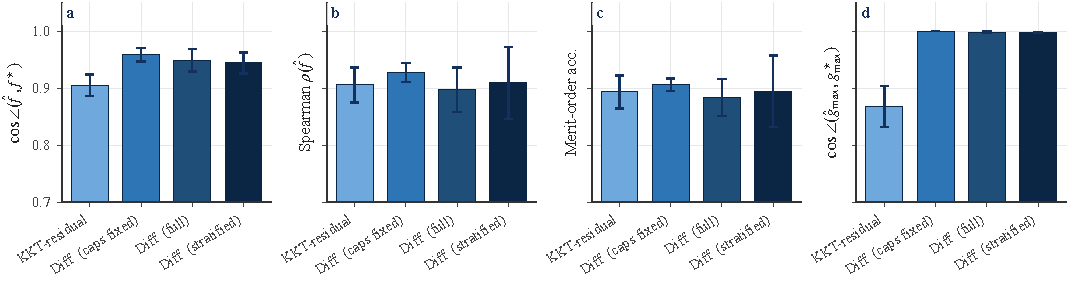
\includegraphics[width=0.96\linewidth]{../paper/figures/methods_recovery.pdf}
    \end{center}
    {\small Cosine, Spearman~$\rho$, and merit-order accuracy on $\hat f$,
    plus cosine on $\hat g_{\max}$.  The differentiable estimator recovers
    capacities almost exactly ($\cos \hat g_{\max} \approx 0.999$) while
    remaining competitive on cost recovery.}
  \end{block}

\end{column}

%% =====================================================================
%% COLUMN 3
%% =====================================================================
\begin{column}{0.295\textwidth}

  % --- Sample/noise sweeps ------------------------------------------
  \begin{block}{Sample-Size \& Noise Robustness}
    \begin{center}
      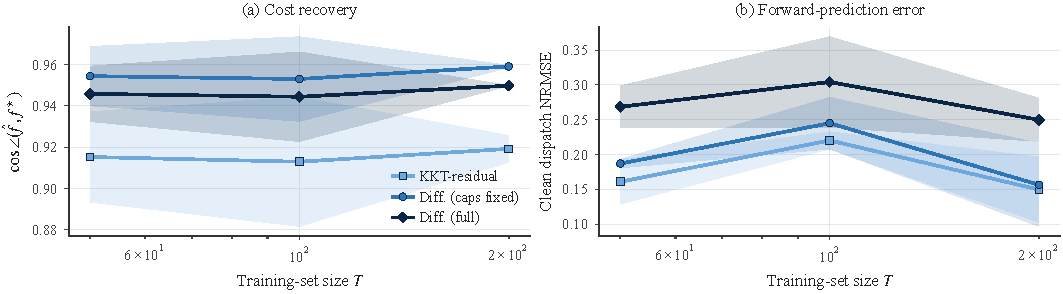
\includegraphics[width=0.95\linewidth]{../paper/figures/sweep_size.pdf}
    \end{center}
    {\small Recovery vs.\ training size $T\in\{50,100,200,400\}$
    (3 seeds; bands = $\pm1\sigma$). Differentiable estimator dominates
    KKT at every $T$.}

    \smallskip
    \begin{center}
      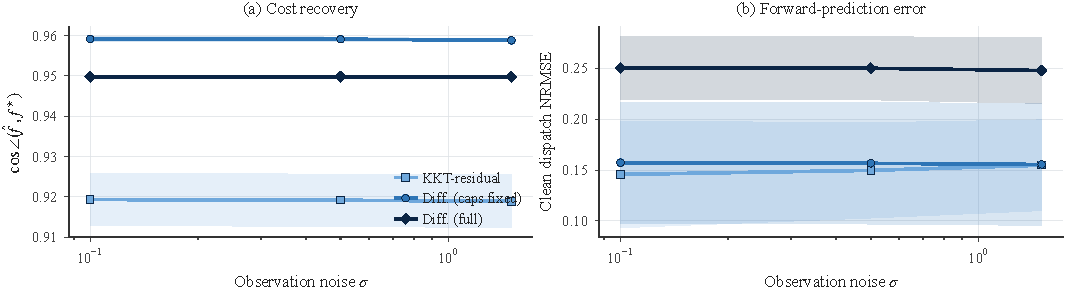
\includegraphics[width=0.95\linewidth]{../paper/figures/sweep_noise.pdf}
    \end{center}
    {\small Recovery vs.\ observation noise $\sigma$ (3 seeds). Gap widens
    under higher noise where the Huber loss provides extra robustness.}
  \end{block}

  % --- Diurnal recovery ---------------------------------------------
  \begin{block}{Diurnal Cost Recovery}
    \begin{center}
      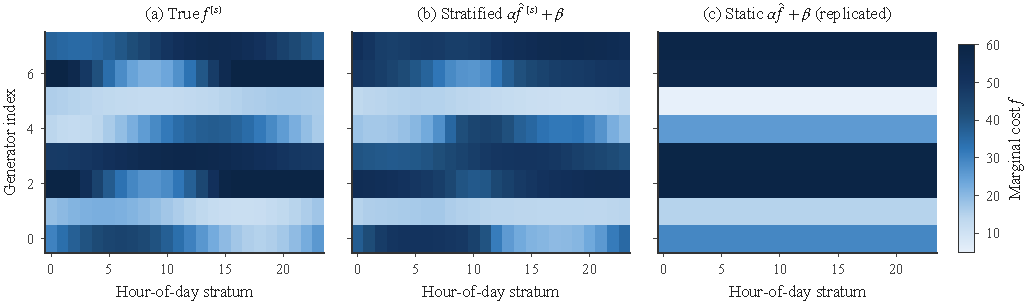
\includegraphics[width=0.95\linewidth]{../paper/figures/diurnal_heatmap.pdf}
    \end{center}
    {\small Hour-of-day cost table for 8-bus network with 60\% diurnal
    cost amplitude. \textbf{Truth} (left) vs.\ \textbf{Stratified}
    (centre) vs.\ \textbf{Static} (right).  The static model collapses
    the diurnal swing; the stratified estimator recovers it faithfully.}
  \end{block}

  % --- MEFs ---------------------------------------------------------
  \begin{block}{Downstream: Marginal Emission Factors}
    Autograd Jacobian $\partial g\opt/\partial d$ enables exact MEFs:
    $\mathrm{MEF}(d) = \nabla_d\bigl(c_{CO_2}^\top g\opt(d)\bigr)$.

    \begin{center}
      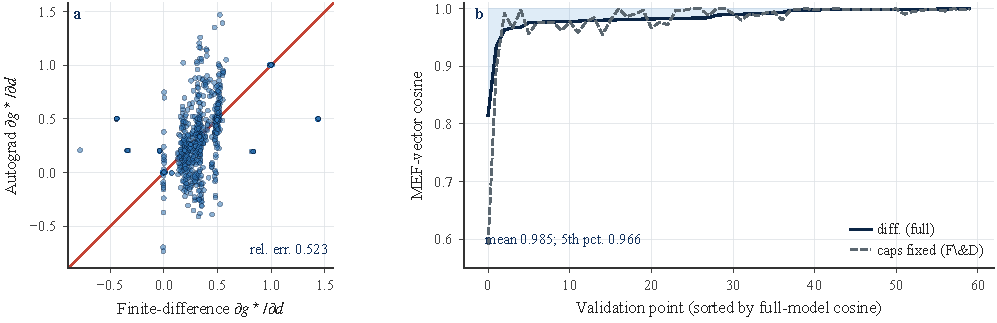
\includegraphics[width=0.95\linewidth]{../paper/figures/mef_validation.pdf}
    \end{center}
    {\small \textbf{(a)} Autograd vs.\ finite-difference Jacobian
    validation. \textbf{(b)} Estimated vs.\ true MEFs; both full and
    caps-fixed estimators achieve \highlight{cosine $0.98$}
    (RMSE $= 0.10$).}
  \end{block}

  % --- Conclusions --------------------------------------------------
  \begin{alertblock}{Conclusions \& Contributions}
    \begin{itemize}
      \item \textbf{Joint recovery:} $\cos\hat f = 0.96$, merit-order
            accuracy $= 0.90$, $\cos\hat g_{\max} \approx 1.00$
            — outperforming KKT on every structural metric
      \item \textbf{9\% lower} clean dispatch NRMSE vs.\ KKT baseline
            with \textbf{5$\times$ tighter} seed variance
      \item \textbf{Stratified model} faithfully captures diurnal
            merit-order swing where static models fail
      \item \textbf{PJM-like validation:} 80\% pairwise merit-order
            accuracy on 8 realistic fuel buckets
      \item \textbf{Exact MEF oracle:} cosine $0.98$ vs.\ truth via
            implicit KKT differentiation
      \item Identifiability lemma + empirical score predict which
            generators are recoverable from data
    \end{itemize}

    \medskip
    \textbf{Future work:} Unit commitment, ramping constraints, learned
    strata, scaling KKT baseline to $T\gtrsim10^4$.
  \end{alertblock}

\end{column}

\end{columns}

\end{frame}
\end{document}
